% === Revised Section 2: Shannon prelude ===
%
% NEW PREAMBLE ADDITIONS NEEDED (add once to the parent document's preamble;
% they are listed here as a comment so this file can be \input{} cleanly):
%
% \usepackage{tikz}
% \usetikzlibrary{trees,positioning,arrows.meta}
% \usepackage{listings}
% \lstset{basicstyle=\ttfamily\small, language=Python,
%         showstringspaces=false, columns=flexible}
%
% \newtcolorbox{activity}[1][]{
%   breakable, enhanced,
%   colback=blue!5, colframe=blue!55!black,
%   coltitle=white, fonttitle=\bfseries,
%   title={Activity},
%   boxrule=0.6pt,
%   left=6pt,right=6pt,top=4pt,bottom=4pt,
%   #1
% }
%
% \newtcolorbox{aside}[1][]{
%   breakable, enhanced,
%   colback=gray!6, colframe=gray!55!black,
%   coltitle=white, fonttitle=\bfseries,
%   title={Aside},
%   boxrule=0.5pt,
%   left=6pt,right=6pt,top=4pt,bottom=4pt,
%   #1
% }
%
% =========================================================================

\section{Prelude: Shannon and the cost of surprise}
\label{sec:shannon-prelude}

\begin{intuition}
Information is the price you pay for being surprised, and you are
surprised in exact proportion to how unlikely an event was. Keep
three numbers in mind for the rest of this section:

\begin{itemize}[leftmargin=2em,itemsep=1pt]
  \item \textbf{Fair coin.} $p(\text{heads}) = \tfrac12$. One yes/no
    question settles it: $H = 1$ bit per flip.
  \item \textbf{Biased coin, 7/8 heads.} Most flips are boring;
    occasionally a tail surprises you. The average surprise works out
    to
    \[
      H = -\tfrac78\log_2\tfrac78 - \tfrac18\log_2\tfrac18
        \;\approx\; 0.169 + 0.375 \;=\; 0.544 \text{ bits per flip}.
    \]
    That is the ``about half a bit'' we promised --- now with the
    arithmetic to back it up.
  \item \textbf{A 1-in-1024 event.} $-\log_2(1/1024) = 10$ bits of
    ``wow.'' A 50/50 event carries one bit of ``huh.''
\end{itemize}

Two forecasters make this concrete. In Los Angeles, Ana says
``sunny'' nearly every day and is right nearly every day; her
distribution over \{sun, cloud, rain\} is roughly
$(0.85, 0.10, 0.05)$, so $H(\text{LA}) \approx 0.74$ bits per day.
In Zurich, B\"arbel faces \{sun, cloud, rain, snow, F\"{o}hn, fog\}
with a distribution closer to $(0.25, 0.30, 0.25, 0.07, 0.03, 0.10)$,
giving $H(\text{ZRH}) \approx 2.32$ bits per day. If the newspaper
pays each forecaster one cent per bit transmitted, B\"arbel earns
about three times what Ana does --- not because Zurich is colder,
but because Zurich is \emph{less predictable}. Shannon's
source-coding theorem (\cref{thm:source-coding}) says neither can do
better than her own entropy floor, no matter how clever her code.

\textbf{Why a decision-maker should care.} Every storage bill, every
bandwidth bill, every ``our model is more efficient'' vendor claim
bottoms out against an entropy floor. Printed English has entropy
between about $0.6$ and $1.3$ bits per character \citep[Ch.~6]{coverthomas2006};
if a vendor tells you they compress English text to $0.3$ bits per
character, they are either wrong, lying, or have discovered English
has lower entropy than anyone thought --- which would itself be news
on the scale of cold fusion. Entropy also sets the floor on
forecasting: no analyst, human or machine, can predict a genuinely
high-entropy process (next week's lottery numbers) better than
chance, no matter how much compute you throw at it. Knowing where
the entropy floor sits for \emph{your} data is the difference
between a reasonable AI budget and a fantasy one.
\end{intuition}

\subsection*{Formal setup}

Fix a finite \emph{alphabet} $\mathcal{A} = \{a_1, \dots, a_K\}$ and
let $X$ be a discrete random variable on $\mathcal{A}$ with
probability mass function $p(a) = \Pr[X = a]$. All logarithms are
base $2$ unless stated; values are measured in \emph{bits}. The
alphabet could be \{heads, tails\} for a coin, \{A, C, G, T\} for a
DNA base, the 256 possible bytes in a file, or the roughly $50{,}000$
sub-word tokens inside a modern language model.

\begin{definition}[Self-information and Shannon entropy]
\label{def:entropy}
The \textbf{self-information} (or \emph{surprisal}) of the outcome
$x \in \mathcal{A}$ under $p$ is
\begin{equation}
  I_p(x) \;=\; -\log_2 p(x),
  \label{eq:self-info}
\end{equation}
with the convention $0 \cdot \log_2 0 = 0$. The \textbf{Shannon
entropy} of $X$ is the expected self-information,
\begin{equation}
  H(X) \;=\; \mathbb{E}\bigl[I_p(X)\bigr]
       \;=\; -\sum_{k=1}^{K} p(a_k)\,\log_2 p(a_k).
  \label{eq:entropy}
\end{equation}
\end{definition}

\begin{aside}[Why the logarithm?]
Three demands pin down $-\log_2 p$ up to the choice of base.
(i) A sure event ($p=1$) should carry zero surprise: $\log 1 = 0$.
(ii) Rarer events should carry more surprise: $-\log p$ is decreasing
in $p$. (iii) Independent surprises should \emph{add}: if $X$ and
$Y$ are independent, the surprise of seeing both is
$-\log(p_X p_Y) = -\log p_X - \log p_Y$. Only the logarithm turns
multiplication of probabilities into addition of surprise, which is
exactly what ``number of yes/no questions'' demands.
\end{aside}

\subsection*{Codes, trees, and Kraft}

A \textbf{code} for $\mathcal{A}$ is an injective map
$C : \mathcal{A} \to \{0,1\}^*$ assigning a binary string $C(a)$ to
each symbol. We write $\ell(a) = |C(a)|$ for the code length. $C$
is a \textbf{prefix code} (or \emph{instantaneous code}) if no
codeword $C(a_i)$ is a proper prefix of any other codeword $C(a_j)$.
The prefix property is what lets a receiver decode a stream of
codewords without delimiters: as soon as the bits read match a
codeword, that codeword is committed.

\begin{figure}[h]
\centering
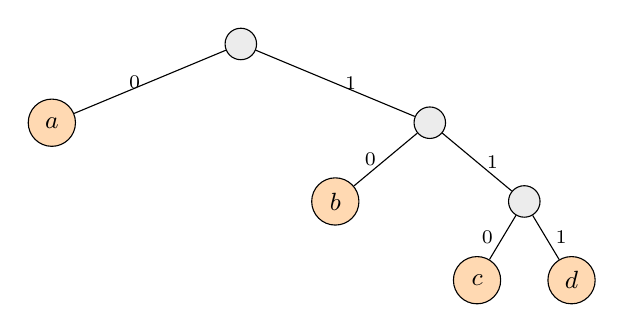
\begin{tikzpicture}[
  level distance=10mm,
  level 1/.style={sibling distance=48mm},
  level 2/.style={sibling distance=24mm},
  level 3/.style={sibling distance=12mm},
  every node/.style={font=\small},
  leaf/.style={draw, circle, fill=orange!30, inner sep=1pt, minimum size=6mm},
  inner/.style={draw, circle, fill=gray!15, inner sep=1pt, minimum size=4mm},
  edgelab/.style={font=\scriptsize, midway}
]
\node[inner] {}
  child {node[leaf] {$a$} edge from parent node[edgelab, left] {$0$}}
  child {node[inner] {}
    child {node[leaf] {$b$} edge from parent node[edgelab, left] {$0$}}
    child {node[inner] {}
      child {node[leaf] {$c$} edge from parent node[edgelab, left] {$0$}}
      child {node[leaf] {$d$} edge from parent node[edgelab, right] {$1$}}
      edge from parent node[edgelab, right] {$1$}
    }
    edge from parent node[edgelab, right] {$1$}
  };
\end{tikzpicture}
\caption{Prefix-code tree for the code $C(a)=0,\ C(b)=10,\
C(c)=110,\ C(d)=111$. Each leaf is a codeword; no codeword lies on
the path to another. The subtree rooted at depth $\ell$ covers a
$2^{-\ell}$ fraction of the infinite leaves, which is the content of
Kraft's inequality.}
\label{fig:prefix-tree}
\end{figure}

\begin{lemma}[Kraft's inequality]
\label{lem:kraft}
For any prefix code $C$ on $\mathcal{A}$ with lengths $\ell(a_k)$,
\begin{equation}
  \sum_{k=1}^{K} 2^{-\ell(a_k)} \;\le\; 1.
  \label{eq:kraft}
\end{equation}
Conversely, for any length assignment $\ell_1, \dots, \ell_K \in
\mathbb{N}$ satisfying~\eqref{eq:kraft} there exists a prefix code
with those lengths.
\end{lemma}

\begin{proof}[Proof sketch]
Identify each codeword with a leaf in the infinite binary tree
(\cref{fig:prefix-tree}). A prefix condition forbids any codeword
from lying on the path to another, so distinct codewords correspond
to \emph{disjoint} subtrees. The subtree rooted at a node of depth
$\ell$ contains a $2^{-\ell}$ fraction of the infinite leaves, and
disjointness of those fractions gives the bound. The converse is an
explicit construction: sort $\ell_k$ in increasing order and assign
the lexicographically smallest available length-$\ell_k$ string at
each step.
\end{proof}

\begin{example}[Entropy of a 4-symbol alphabet, revisited early]
\label{ex:h4}
Let $\mathcal{A} = \{a, b, c, d\}$ with $p(a) = \tfrac{1}{2}$,
$p(b) = \tfrac{1}{4}$, $p(c) = p(d) = \tfrac{1}{8}$. Then
\begin{align*}
  H(X) &= -\tfrac{1}{2}\log_2\tfrac{1}{2}
         - \tfrac{1}{4}\log_2\tfrac{1}{4}
         - 2\cdot\tfrac{1}{8}\log_2\tfrac{1}{8} \\
       &= \tfrac{1}{2}\cdot 1 + \tfrac{1}{4}\cdot 2 + \tfrac{1}{4}\cdot 3
        \;=\; \tfrac{7}{4} \text{ bits}.
\end{align*}
The prefix code $C(a) = 0,\ C(b) = 10,\ C(c) = 110,\ C(d) = 111$ of
\cref{fig:prefix-tree} achieves expected length
$L = \tfrac12\cdot 1 + \tfrac14\cdot 2 + \tfrac18\cdot 3 + \tfrac18\cdot 3
= \tfrac74$ bits exactly. Its lengths $(1,2,3,3)$ satisfy Kraft with
\emph{equality} and match $-\log_2 p(a_k)$ symbol by symbol. When
probabilities are negative powers of two, the Shannon floor is hit on
the nose.
\end{example}

\begin{activity}[Guess-the-next-flip bet game --- 10 minutes]
\label{act:bet}
Pair students up. One student flips a coin biased 3/4 heads
(simulated by rolling a d4: 1--3 $=$ heads, 4 $=$ tails); the other
bets any fraction of a running 16-chip stake on the outcome. The
house rule: if you bet fraction $f$ on the outcome that actually
occurs and the true probability was $p$, your stake is multiplied by
$2f/(2p) = f/p$.\footnote{The Kelly-optimal fraction is $f=p$, which
multiplies the stake by $1$ on average; deviations lose in the long
run. Over many rounds the log-growth rate is
$\sum_x q(x)\log_2(f(x)/p(x))$, a KL divergence.}
Play ten rounds, then compute per round
\[
  \text{(avg. chips lost)} \;\approx\; D_{\mathrm{KL}}(p \,\|\, q)
  \;=\; \sum_x p(x)\log_2\tfrac{p(x)}{q(x)},
\]
where $q$ is the student's betting distribution. The class discovers
\emph{experimentally} that the only way not to bleed chips is to bet
$q = p$, and that their average loss equals the gap between the
cross-entropy they ``paid'' and Shannon's floor $H(p)$.
\textit{Leo:} a scoreboard he can compute round by round.
\textit{Yuki:} bits become chips.
\end{activity}

\subsection*{Gibbs' inequality: the wrong code pays a tax}

\begin{lemma}[Gibbs' inequality]
\label{lem:gibbs}
For any two probability mass functions $p, q$ on $\mathcal{A}$,
\begin{equation}
  -\sum_{k} p(a_k) \log_2 q(a_k)
    \;\ge\; -\sum_{k} p(a_k) \log_2 p(a_k),
  \label{eq:gibbs}
\end{equation}
with equality if and only if $p = q$.
\end{lemma}

\begin{aside}[A one-picture reason to believe $\ln x \le x - 1$]
The curve $y = \ln x$ is concave; its tangent at $x = 1$ is the line
$y = x - 1$. A concave curve lies on or below any of its tangents,
so $\ln x \le x - 1$ everywhere, with equality exactly at $x = 1$.
Draw the two curves on the same axes once; you will never forget
this inequality again.
\end{aside}

\begin{proof}
Using $\ln x \le x - 1$ (with equality iff $x = 1$) and
$\log_2 x = \ln x / \ln 2$,
\[
  \sum_k p(a_k) \log_2 \frac{q(a_k)}{p(a_k)}
  \;\le\; \frac{1}{\ln 2}\sum_k p(a_k)\!\left(\frac{q(a_k)}{p(a_k)} - 1\right)
  \;=\; \frac{1}{\ln 2}\Bigl(\sum_k q(a_k) - 1\Bigr) \;\le\; 0,
\]
because $\sum_k q(a_k) \le 1$. Rearranging gives~\eqref{eq:gibbs};
the equality conditions of $\ln x \le x - 1$ and $\sum q = 1$
together force $p = q$.
\end{proof}

\begin{intuition}[What Gibbs really says]
If the world is distributed as $p$ but you design a code as if the
world were distributed as $q$, you pay $-\sum p\log q$ bits on
average instead of $-\sum p\log p$. The difference,
\[
  D_{\mathrm{KL}}(p \,\|\, q)
    \;=\; \sum_k p(a_k) \log_2 \tfrac{p(a_k)}{q(a_k)},
\]
is the \emph{tax} the world levies on your wrong model. It is
non-negative, zero only when $q=p$, and we will meet it again under
the name ``cross-entropy loss'' whenever a neural network is being
trained.
\end{intuition}

\subsection*{Shannon's source-coding theorem}

\begin{theorem}[Shannon source-coding inequality]
\label{thm:source-coding}
Let $C$ be any uniquely decodable (in particular, any prefix) code
for $\mathcal{A}$ and let $L = \mathbb{E}[\ell(X)] =
\sum_k p(a_k)\ell(a_k)$ be its expected code length. Then
\begin{equation}
  L \;\ge\; H(X).
  \label{eq:source-coding}
\end{equation}
Moreover, there exists a prefix code (e.g.\ the Shannon--Fano code
with $\ell(a_k) = \lceil -\log_2 p(a_k)\rceil$) such that
\begin{equation}
  L \;<\; H(X) + 1.
  \label{eq:source-coding-achiev}
\end{equation}
\end{theorem}

\begin{proof}[Proof sketch]
Let $q(a_k) = 2^{-\ell(a_k)} / Z$, where
$Z = \sum_k 2^{-\ell(a_k)} \le 1$ by \cref{lem:kraft}; so $q$ is a
bona fide probability vector. Read $q$ as the \emph{implicit model}
your code $C$ is betting on: it assigns probability $q(a_k)$ to
symbol $a_k$ because it spent $\ell(a_k)$ bits describing it. By
\cref{lem:gibbs}, the cross-entropy $-\sum_k p(a_k) \log_2 q(a_k)
\ge H(X)$, i.e.\ the wrong model pays a tax. Because
$-\log_2 q(a_k) = \ell(a_k) + \log_2 Z \le \ell(a_k)$ (since $Z \le
1$ makes $\log_2 Z \le 0$), we get $L \ge -\sum_k p(a_k)\log_2
q(a_k) \ge H(X)$. For~\eqref{eq:source-coding-achiev}, the lengths
$\lceil -\log_2 p(a_k)\rceil$ satisfy Kraft~\eqref{eq:kraft}, and
each ceiling adds at most $1$ to the expected length. See
\citet[Ch.~5]{coverthomas2006} for the full treatment.
\end{proof}

\begin{aside}[The slogan, properly qualified]
``Every code is a probability model and every probability model is a
code.'' Precisely: a prefix code with lengths $\ell(a_k)$ implicitly
asserts the distribution $q(a_k) \propto 2^{-\ell(a_k)}$; a
distribution $q$ suggests lengths $\lceil -\log_2 q(a_k)\rceil$.
When we train a language model to minimise cross-entropy loss, we
are literally minimising the expected code length under Shannon's
theorem. This is the hinge that the rest of these notes turns on.
\end{aside}

\subsection*{More worked examples}

\begin{example}[Back to the 4-symbol alphabet, with a wrong model]
\label{ex:h4-wrong}
Keep $p = (\tfrac12, \tfrac14, \tfrac18, \tfrac18)$ but design a code
as if the distribution were uniform, $q = (\tfrac14, \tfrac14,
\tfrac14, \tfrac14)$, giving two bits per symbol to every letter.
Then $L = 2$ bits, the cross-entropy is $-\sum p \log_2 q = 2$ bits,
and the KL tax is $D_{\mathrm{KL}}(p\|q) = 2 - \tfrac74 = \tfrac14$
bit per symbol. Over a million symbols, betting on uniform instead
of $p$ costs you $250{,}000$ bits --- about $31$ kilobytes of
wasted bandwidth.
\end{example}

\begin{example}[Biased coin, bit by bit]
\label{ex:biased-coin}
The $7/8$-heads coin has $H \approx 0.544$ bits. You cannot encode
one flip in fewer than one bit, of course --- codewords are
integer-length. But if you block flips in groups of $10$, the
block alphabet has $2^{10} = 1024$ outcomes and the block entropy
is $10\cdot 0.544 = 5.44$ bits, which Shannon--Fano reaches to
within one bit. Long-run bandwidth drops from $10$ bits per block
(naive) to about $6$ bits per block. This is why every real
compressor (gzip, arithmetic coding, LLM tokenisers) works on
blocks or streams, not symbol-by-symbol.
\end{example}

\begin{activity}[Entropy of your phone lock-screen --- 5 minutes]
\label{act:pin}
On scrap paper, write down (1) the length $n$ of your phone PIN or
pattern, (2) whether it contains a birthday (your own, a partner's,
a child's), and (3) whether it repeats a digit. Using the prior
\[
  p(\text{PIN}) \approx
  \begin{cases}
    3\times 10^{-3} & \text{if birthday-shaped}, \\
    10^{-n}          & \text{otherwise},
  \end{cases}
\]
compute $-\log_2 p$ in bits. Compare to the entropy of a uniformly
random $n$-digit PIN, $n \log_2 10 \approx 3.32 n$ bits. The typical
result in a classroom is that ``birthday'' PINs land near $8$--$9$
bits while a truly random 6-digit PIN is near $20$ bits. That
$\sim 11$-bit gap is the factor-of-$2000$ advantage a thief enjoys
against the average human.
\textit{Yuki:} personally concrete. \textit{Leo:} ends in a number.
\end{activity}

\begin{activity}[Huffman-code-by-hand worksheet --- 15 minutes]
\label{act:huffman}
Given probabilities $p = (0.40, 0.20, 0.15, 0.15, 0.10)$ over
symbols $\{A,B,C,D,E\}$:
\begin{enumerate}[leftmargin=2em,itemsep=1pt]
  \item Sort and repeatedly merge the two lowest-probability symbols
    into a meta-symbol whose probability is their sum. Record each
    merge as a parent node.
  \item After four merges you have a single root. Label each left
    edge $0$ and each right edge $1$; read each leaf's codeword
    from the root.
  \item Compute $L = \sum p(a_k) \ell(a_k)$ and compare to
    $H(X) = -\sum p \log_2 p \approx 2.15$ bits. The Huffman code
    achieves $L = 2.20$ bits, within $0.05$ of entropy.
  \item \textit{Stretch:} change $p(A)$ from $0.40$ to $0.95$ and
    redo. Watch the code for $A$ collapse to a single bit while the
    others grow. This is the shape of \emph{adaptive} compression.
\end{enumerate}
\textit{Leo:} pencil-and-paper payoff. \textit{Yuki:} the tree
becomes a physical drawing.
\end{activity}

\begin{activity}[Six lines of Python --- take home]
\label{act:python}
Paste this into any Python 3 prompt:
\begin{verbatim}
from collections import Counter
from math import log2
def H(s):
    n = len(s)
    return -sum((c/n)*log2(c/n) for c in Counter(s).values())
print(H("to be or not to be that is the question"))
\end{verbatim}
Run it on (a) the first paragraph of a novel in your native
language, (b) the same paragraph translated to English, and (c) a
200-character string of your own keystrokes. You will typically see
$H \approx 4.2$ bits per character on natural-language prose and
$H \approx 3.0$ on keystrokes from a human who has a strong
hand-preference. The true entropy of English is lower
(${\sim}1$ bit/char) because this snippet ignores correlations
between neighbouring characters --- which is exactly the gap a
language model closes.
\textit{Leo:} code he can execute. \textit{Yuki:} numbers for two
inputs he already cares about.
\end{activity}

\begin{aside}[Forward pointer]
We will re-encounter cross-entropy in \cref{def:entropy}'s shadow
every time a neural network is trained; the KL tax will reappear as
the ``surprise'' of a held-out document under a language model; and
the source-coding theorem will become the statement that
\emph{prediction is compression} in the very next section.
\end{aside}
